\documentclass{article}
\usepackage[utf8]{inputenc}
\usepackage{indentfirst}
\usepackage{amsmath}
\usepackage{amssymb}
\usepackage{graphicx}
\usepackage{appendix}
\usepackage{subcaption}
\usepackage{hyperref}
\usepackage{titling}
\usepackage{verbatim}
%\usepackage{wrapfig}

\title{Development of Neural Networks for Learning The Boltzmann Equation	 }
\author{Thomas V Nguyen \\ \\ Department of Mathematics, CSUN, Northridge, CA 91303 \\
	Advisor: Professor Alexander M. Alekseenko
}
\date{}

\begin{document}
\begin{titlepage}
	\maketitle
\end{titlepage}

\section*{Abstract} During the past decades, there are different methods that have been developed to solve the Boltzmann equation: the direct simulation Monte Carlo (DSMC) method, the lattice Boltzmann method (LBM), and the direct deterministic method for computing the Boltzmann equation. In this paper, we explore the physical aspect of the Boltzmann equation and the novel neural network methods for learning the solutions and solving the spatially homogeneous Boltzmann equation.
\section{Introduction} \label{Intro}
The Boltzmann equation describes the statistical behavior of a system of rarefied gases in the non-equilibrium, nonlinear state. The equation analyzes a probability distribution $f(t,\vec{x}, \vec{v})$ for the position and velocity of a typical particle in the small region of $d^3x$ and a small region $d^3v$ of velocity space. The Boltzmann equation is a nonlinear integral differential equation and the unknown function in the equation is a probability density function $f(t,\vec{x}, \vec{v})$ in six-dimensional space of a particle position and velocity and the function $f(t,\vec{x}, \vec{v})$ is evolved in time t. Exact solutions to the Boltzmann equations have been difficult to obtain and is not generally usable in practical problems until the advent of computer technology and numerical analysis methods. Numerically, there have been two development methods of simulating and solving the Boltzmann equation: stochastic and deterministic methods. 

For the stochastic methods, the direct simulation Monte (DSMC) method has been widely used. The DSMC method was first introduced by G.A. Bird in 1963 \cite{BirdGA1} and have been a popular method for numerical simulation of rarefied gas flows. This method randomly generates the number of simulated particles and tracking the binary collisions among the simulated particles to reproduce the underlying physics of the Boltzmann equation. The popular of the DSMC is due to the combination of accuracy, simplicity, and computational efficiency. Beside the Bird’s original method, There are different implementations of DSMC method have developed as described in \cite{DSMC1, DSMC2, DSMC3}. 

The deterministic method of solving the Boltzmann equation is suitable for parallel processing for the computer system that have many CPU cores. One of the deterministic method of solving the Boltzmann equation is the Lattice-Boltzmann method (LBM )as described in the \cite{LBM1, LBM2}. The objective of the LBM methods is to provide simpler model equations for rarefied gas dynamics. Another deterministic method of solving Boltzmann equation is called the discontinuous Galerkin (DG) velocity approximations that can accommodate for the functions discontinuities. \cite{Alekseenko1, Alekseenko2} explored the high order DG discretization using the Gauss quadrature nodes and the Lagrange polynomial basis functions. \cite{Alekseenko4} used the Discrete Fourier Transform to compute the DG approximation for the Boltzmann solution. One can refer \cite{VVAristo} to study the different direct methods for solving the Boltzmann Equation.

In this paper, we will develop a novel method by applying the machine learning and neural networks methodologies to learn the solutions of Boltzmann equation. Specifically, we will construct and train the autoencoders to learn the solutions of Boltzmann equations, construct and train the convolutional neural networks to learn the collision operator, and use the trained convolutional neural network to numerically solve the spatially homogeneous Boltzmann equation based on Euler method. This paper is organized as follow:
\begin{itemize}
	\item Section 2 describes the gas kinetic assumptions and the brief derivation of the Boltzmann equation and its applications.
	\item Section 3 describes the deterministic method for obtaining the solutions of the Boltzmann equation as discussed in \cite{Alekseenko2, Alekseenko4}.
	\item Section 4 describes the general neural network architecture, specifically the fully-connected neural (FCNN) network and convolutional neural network (CNN).
	\item section 5 describes the structure of the solution dataset that is used for training the FCNN and CNN neural networks, the results of training the FCNN to learn the Boltzmann equation's solutions, the results of training CNN networks to learn the collision operator, and using the trained CNN to numerically solve the spatially homogeneous Boltzmann equation.
	\item Section 6 discusses the time efficiency for predicting the solutions of Boltzmann equation and estimate memory requirements for the trained autoencoder and convolutional neural networks.
\end{itemize}

\section{The Boltzmann Equation and its application}
In this section, we briefly describe the derivation of the Boltzmann equation so that we can understand the physical meaning of the Boltzmann equation. One can check \cite{RarefiedGasD, IntroBoltz} for the detail of derivation of the Boltzmann equation.
\subsection{The rarefied gas assumptions}
The Boltzmann equation is derived with the following assumptions of the kinetic theory of gases:
\begin{itemize}
\item Gas consists of very small particles known as molecules having the same mass.
\item The motion of the molecules can be described by Newtonian mechanics.
\item The number of molecules is so large that statistics can be applied.
\item The total volume of the individual gas molecules added up is negligible compared to the volume of the container. Hence, only binary collisions occur between molecules and collisions are perfectly elastic. Kinetic energy and momentum are conserved.
\item The elapsed time of a collision between a molecule and the container's wall is negligible when compared to the time between successive collisions.
\end{itemize}
\subsection{The Boltzmann equation} \label{BoltzEq}
The Boltzmann equation analyzes a probability distribution $f(t, \vec{x}, \vec{v})$ of a particle in a small cell of $(\vec{x}, \vec{v})=(x,y,z,v_x,v_y,v_z)$ evolves with time $t$ in a non-equilibrium state. Suppose at time $t$, particles are in a cell $(\vec{x},\vec{v})$. If an external force $\vec{\textbf{F}}$ instantly acts on each particle causing particles changing in position after $\Delta t$, we have 
\begin{equation} \label{BoltzEqGeneral}
\frac{\partial f}{\partial t} + \vec{v}\cdot\nabla_{\vec{x}}f + \frac{\vec{\textbf{F}}}{m}\cdot\nabla_{\vec{x}}f = \left(\frac{\partial f}{\partial t}\right)_{collision} = I[f](t,\vec{x},\vec{v})
\end{equation}
If there is no external force $\vec{\textbf{F}} = 0$, then (1) is written as:
\begin{equation} \label{BoltzEqNoForce}
\frac{\partial f}{\partial t} + \vec{v}\cdot\nabla_{\vec{x}}f = I[f](t,\vec{x},\vec{v})
\end{equation}
Here $I[f](t,\vec{x},\vec{v})$ is the molecular collision operator. For binary collisions between molecules, the collision operator takes the form:
\begin{multline} \label{CollOp}
I[f](t,\vec{x},\vec{v}) = \\ \int_{\mathbb{R}^3}\int_{\mathbb{S}^2}(f(t,\vec{x},\vec{v}^\prime)f(t,\vec{x},\vec{u}^\prime) - f(t,\vec{x},\vec{v})f(t,\vec{x},\vec{u}))B(|g|,\cos\theta)d\sigma d\vec{u}
\end{multline}
Where
\begin{itemize}
	\item $\vec{v}$ and $\vec{u}$ are the pre-collision velocities of a pair of molecules.
	\item $\vec{g} = \vec{v} - \vec{u}$.
	\item $\mathbb{S}^2$ is a unit sphere in $\mathbb{R}^3$ centered at the origin.
	\item $\vec{w}$ is the unit vector connecting the origin and a point on $\mathbb{S}^2$.
	\item $\theta$ is the deflection angle defined by the equation $\cos\theta = \vec{w}\cdot\vec{g}/|g|$.
	\item $d\theta = sin\theta d\theta d\varepsilon$ where $\varepsilon$ is the azimuthal angle parametrizes $\vec{w}$ together with the angle $\theta$.
	\item $\vec{v}$ and $\vec{u}$ are the post-collision velocities of a pair of particles and are computed by
	\begin{equation*}
		\vec{v}^\prime = \vec{v} - \frac{1}{2}(\vec{g} - |g|\vec{w}), \quad \vec{u}^\prime = \vec{v} - \frac{1}{2}(\vec{g} - |g|\vec{w})
	\end{equation*}
	\item The kernel $B(|g|,\cos\theta)$ characterizes interactions of the molecules and is selected appropriately to reproduce the desired characteristics of the gas.
\end{itemize}

For the spatially homogeneous relaxation problem, we assume that the distribution density function of molecular velocities $f(t, \vec{x}, \vec{v})$ is constant in the spatial variable $\vec{x}$, i.e., $f(t, \vec{x}, \vec{v}) = f(t, \vec{v})$. Then the derivative of solution with respect to $\vec{x}$ vanishes and the spatially homogeneous form of the Boltzmann equation is:
\begin{equation}	\label{BoltzHomo}
	\frac{\partial}{\partial t}f(t,\vec{v}) = I[f](t, \vec{v})
\end{equation}
Solving and learning solutions of the spatially homogeneous quation \ref{BoltzHomo} is the main discussion in this paper. We will discuss briefly how to solve equation \ref{BoltzHomo} numerically in section \ref{DGSol} to obtain the solution dataset and how the solution dataset is used to train the neural networks to learn the solution data and collision operator.
\subsection{The Boltzmann equation's applications}
Below are the applications of the Boltzmann equation:
\begin{itemize}
	\item The Boltzmann equation is a foundation for deriving the theory of thermodynamics and kinetic theory of gasses.
	\item The Boltzmann equation can be used to determine how physical quantities change, such as heat energy and momentum, when a fluid is in transport. One may also derive other properties characteristic to fluids such as thermal.
	\item In the advent of hypersonic flight, flows in satellite electric propulsion thrusters and around thrusters, and in re-entry from space flight, the Boltzmann equation can be used to describe accurately for these aerodynamics flights in rarefied gas regimes.
\end{itemize}

\section{Deterministic Numerical solutions for the Boltzmann equation and the solution dataset} \label{BoltzSol}
In this section, we will briefly describe the numerical methods of obtaining the solutions of the Boltzmann equation. One can refer to \cite{Alekseenko2, Alekseenko4} for the detail of these methods. We will then describe the solution data set obtained by these two numerical methods. The solution data set will be used in section \ref{NN} for learning the solutions of Boltzmann equation.
\subsection{Deterministic solution of the spatially homogeneous Boltzmann equation using discontinuous Galerkin discritization in the velocity space} \label{DGSol}
To evaluate the collision operator in equation (\ref{BoltzHomo}), as described in \cite{Alekseenko2}, we select a rectangular parallelepiped in the velocity space  and partition this region into parallelepipeds $K_j$. Let $\vec{v} = (u,v,w)$ and let $s_u, s_v, s_w$ be the degrees of the polynomial basis functions in the velocity components $u, v$ and $w$ respectively. Let $K_j = [u^L_j, u^R_j]\times[v^L_j,v^R_j]\times[w^L_j,w^R_j]$. We construct the Lagrange basis functions as follows:

We introduce the nodes of Gauss quadratures of orders $s_u, s_v$ and $s_w$ on each of the intervals $[u^L_j,u^R_j], [v^L_j,v^R_j]$ and $[w^L_j, w^R_j]$ respectively. Let these nodes be denoted $\kappa^u_{p;j}, p=1,\dots,s_u, \kappa^v_{q;j} q=1,\dots,s_v$ and $\kappa^w_{r;j}, r=1,\dots,s_w$. Then the Lagrange basis functions are defined as:
\begin{equation*}
\phi^u_{l;j} = \prod_{\substack{p=1,s^u \\ p \neq l}}\frac{\kappa^u_{p;j} - u}{\kappa^u_{p;j} - \kappa^u_{l;j}}, \quad \phi^v_{m;j} = \prod_{\substack{q=1,s^v \\ 1 \neq m}}\frac{\kappa^v_{q;j} - u}{\kappa^v_{q;j} - \kappa^v_{m;j}}, \quad \phi^w_{r;j} = \prod_{\substack{r=1,s^w \\ p \neq n}}\frac{\kappa^w_{r;j} - w}{\kappa^w_{r;j} - \kappa^w_{n;j}}
\end{equation*}
The three-dimensional basis functions are given as
\begin{equation}
	\phi_{i;j}(\vec{v})= \phi^u_{l;j}(u)\phi^v_{m;j}(v)\phi^w_{n;j}(w)
\end{equation} 
Where $i = 1,\dots,s:=s_us_vs_w$ is the index running through all combinations of $l, n and m$.
The following identities hold for basis function $\phi_{i;j}(\vec{v})$:
\begin{equation}
\int_{K_j}\phi_{p;j}(\vec{v})d\vec{v}= \frac{\omega_p\Delta\vec{v}^j}{8}\delta_{pq} \quad and\quad \int_{K_j}\vec{v}\phi_{p;j}(\vec{v})d\vec{v}= \frac{w_p\Delta\vec{v}^j}{8}\vec{v}_{p;j}\delta_{pq}
\end{equation}
where indices $p$ and $q$ run over all combinations of $l, n, and m$ in three dimensional basis functions $\phi_{i;j}(\vec{v})= \phi^u_{l;j}(u)\phi^v_{m;j}(v)\phi^w_{n;j}(w)$ and the vectors $\vec{v}_{p;j}=(\kappa^u_{l;j},\kappa^v_{m;j},\kappa^w_{n;j})$. $\Delta\vec{v}^j=(u^R_j - u^L_j)(v^R_j - v^L_j)(w^R_j - w^L_j)$ and $w_i = w^{s_u}_lw^{s_v}_mw^{s_w}_n$, where $w^{s_u}_l, w^{s_v}_m and w^{s_w}_n$ are the weights of the Gauss quadratures of orders $s_u, s_v and s_w respectively.$
For each $K_i$, the solution for Boltzmann equation can be written in the nodal-DG velocity discetization as:
\begin{equation}
	f(t,\vec{x},\vec{v})|_{K_i} = \sum_{i=1s}f_{i;j}(t,\vec{x})\phi_{i,j}(\vec{v})
\end{equation}
Repeating this for all $K_j$, we can write (\ref{BoltzEqGeneral}) in the numerical form:
\begin{equation}
\partial_tf_{i;j}(t,\vec{x}) + \vec{v}_{i,j}\cdot\nabla_xf_{i,j}(t,\vec{x}) = \frac{8}{w_i\delta\vec{v}^j}I_{\phi_{i;j}}
\end{equation}
with 
\begin{equation} \label{directColl}
I_{\phi_{i;j}} = \int_{\mathbb{R}^3}\int_{\mathbb{R}^3}f(t,\vec{x},\vec{v})f(t,\vec{x},\vec{v}_1)A(\vec{v},\vec{v}_1;\phi_{i;j})d\vec{v}_1d\vec{v}
\end{equation}
where
\begin{equation} \label{kernelA}
	A(\vec{v},\vec{v}_1;\phi_{i;j}) = |g|^\alpha\int_{\mathbb{S}^2}(\phi_{i;j}(\vec{v}') - \phi_{i;j}(\vec{v}))b_\alpha d\sigma
\end{equation}
In \cite{Alekseenko1,Alekseenko2} a nodal dicontinuous Galerkin (DG) discretization of the collision operator leads to a $O(N^{\frac{8}{3}})$ operations where $N$ is the total number of discrete velocity points.
The operator $A(\vec{v},\vec{v}_1;\phi_{i;j})$ in (\ref{kernelA}) has the shift invariant property:
\begin{equation}
A(\vec{v}+\xi,\vec{v}_1+\xi;\phi_{i;j}(\vec{v}-\xi)) = A(\vec{v},\vec{v}_1;\phi_{i;j}) \quad \forall\xi \in \mathbb{R}^3
\end{equation}
With the shift invariant property, we can obtain a bilinear convolution as:
\begin{equation} \label{Convo}
I_i(\vec{\xi}) = \int_{\mathbb{R}^3}\int_{\mathbb{R}^3}f(t,\vec{x},\vec{v} - \vec{\xi})f(t,\vec{v}_1 - \vec{\xi})A(\vec{v},\vec{v}_1;\phi_{i;c})d\vec{v}d\vec{v}_1
\end{equation}
The convolution formular (\ref{Convo}) is used in \cite{Alekseenko4} to develop an $O(N^2)$ method using discrete Fourier transform.

\section{Neural networks architectures} \label{NN}
In this section, we will describe a general architecture of a neural network. How the gradient descent and back propagation algorithms are used to train a neural network to obtain the weights of a neural network. Specifically, we will describe two neural networks that are used to learn the Boltzmann equation solutions and collision operator: the fully connected neural network and convolutional neural network.
\subsection{A general fully connected neural network architecture } \label{FCNN}
A general neural network composes of an input layer, a stack of hidden layers, and an output layer as shown in Figure \ref{fig:NN} which has two hidden layers. Figure \ref{fig:NN} is called a fully connected neural network because each neuron in a hidden layer is connected to all the neurons in the previous layer.
\begin{figure}[h]
	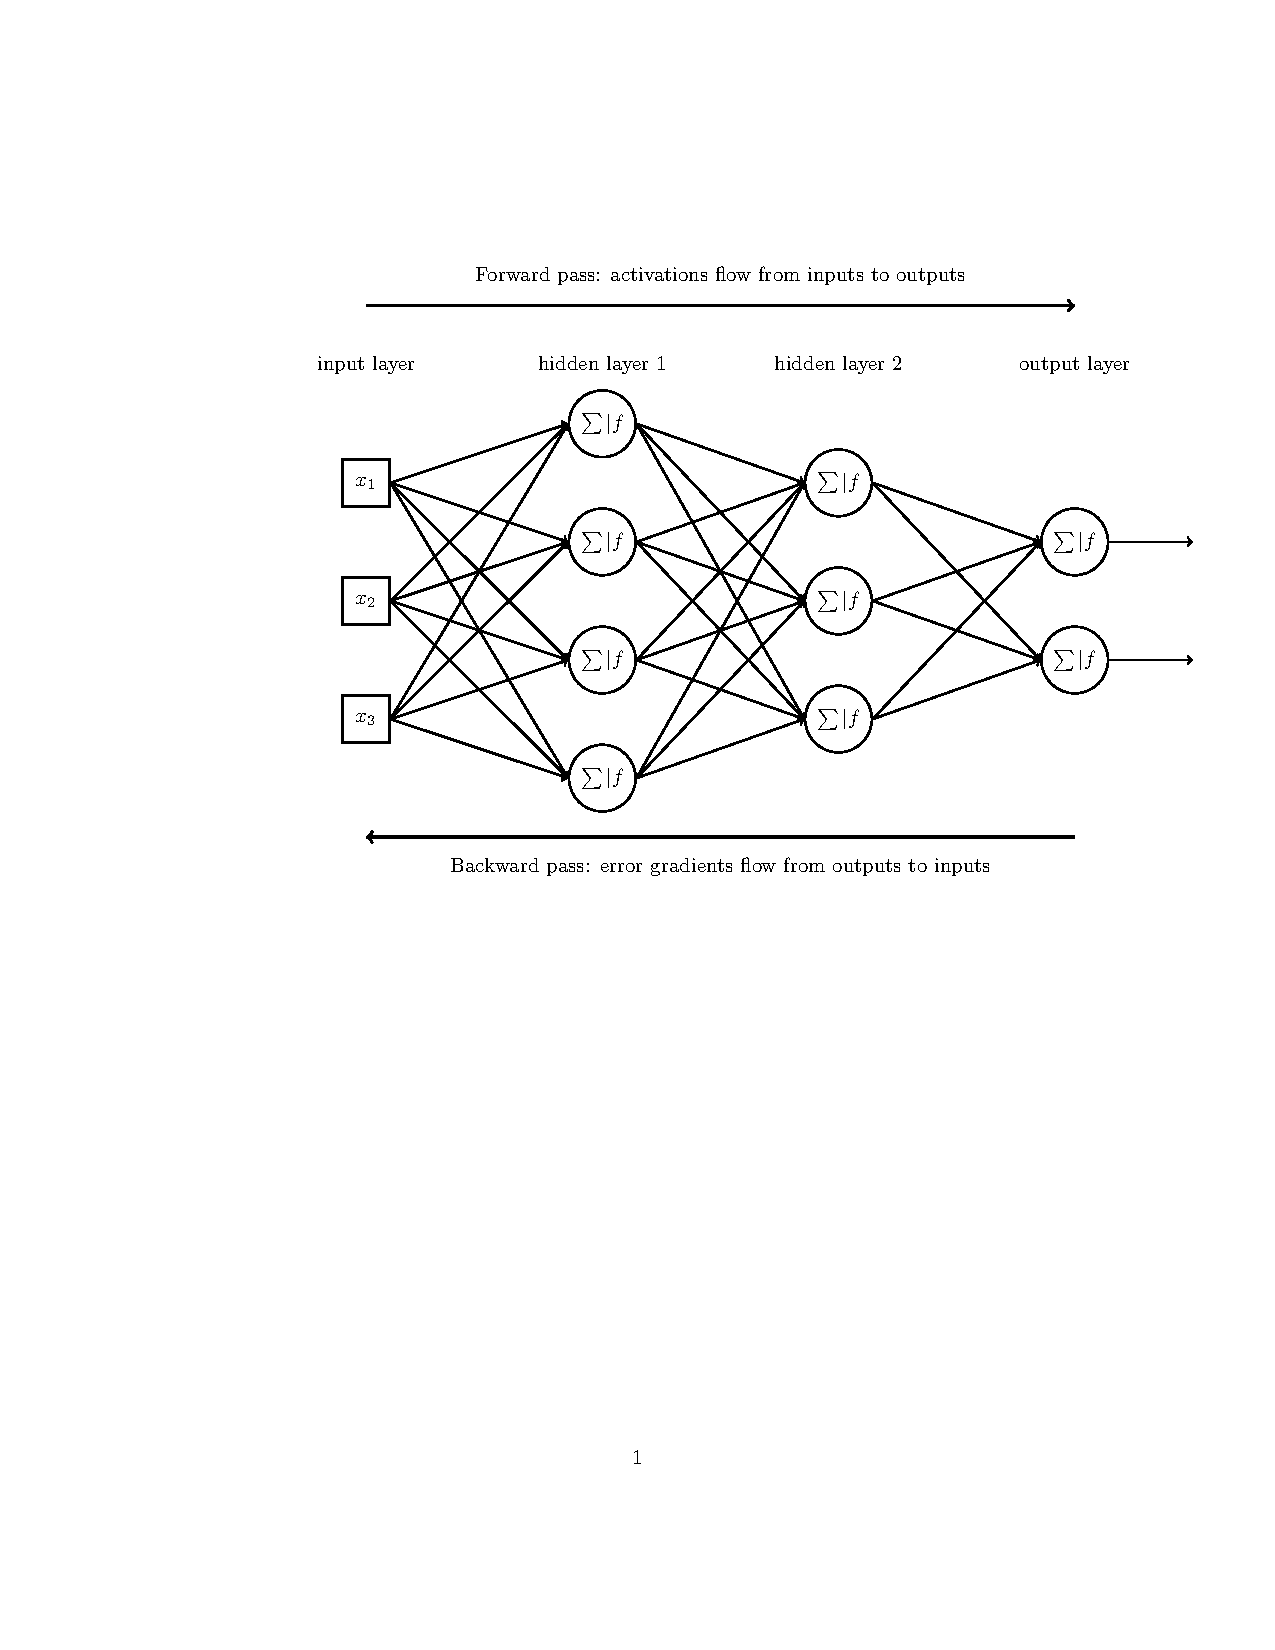
\includegraphics[width=.75\textwidth]{NN.pdf}
	\caption{A general neural network architecture}
	\label{fig:NN}
\end{figure}
A typical neural network may have many hidden layers. Each hidden layer consists of number of neuron and the outputs of each neuron are connected to the inputs of the neurons of the next layer.
The figure \ref{fig:neuron} shows the components of a neuron. 
\begin{figure}[h]
\centering
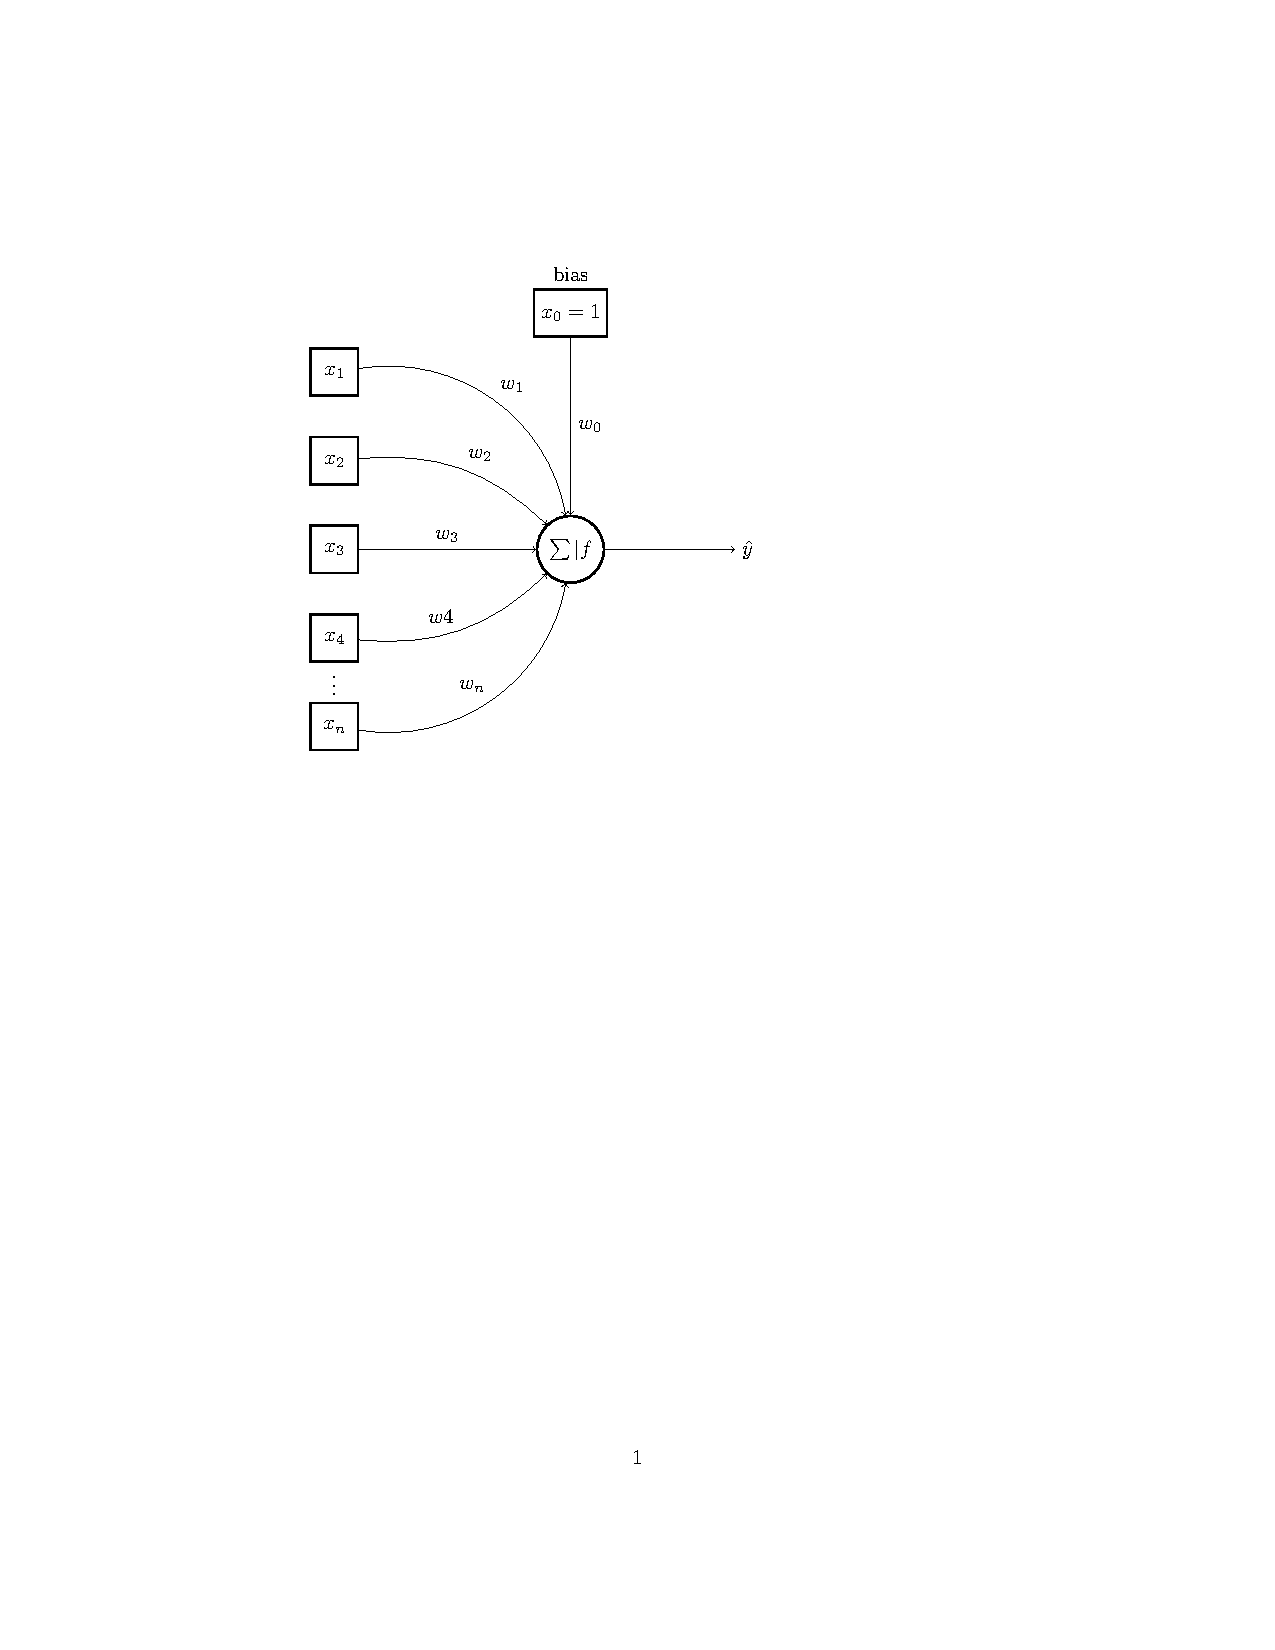
\includegraphics[width=.75\textwidth]{Neuron.pdf}	
\caption{A neurol architecture}
\label{fig:neuron}
\end{figure}

As shown in Figure \ref{fig:neuron}, a neuron receives n inputs $[x_1,x_2, \dots, x_n]$. Each input $x_i$ is associated with a weight $w_i$ and the sum is computed by multiply each input $x_i$ by its associated weight $w_i$ and then sum the resulting values. The result of the weighted sum is then passed into the activation function $f$. Mathematically, we can express these calculations as:
\begin{equation} \label{neuronfunc}
\hat{y} = f\left(\sum_{i=0}^{n}x_i \times w_i\right) = f(z)
\end{equation}
Figure \ref{fig:actFuncs} shows the popular activation functions. Recently, the rectified linear unit function (ReLU) has become the default activation function due to it works well and fast to compute despite it is not differentiable at 0.
\begin{figure}[h]
\centering
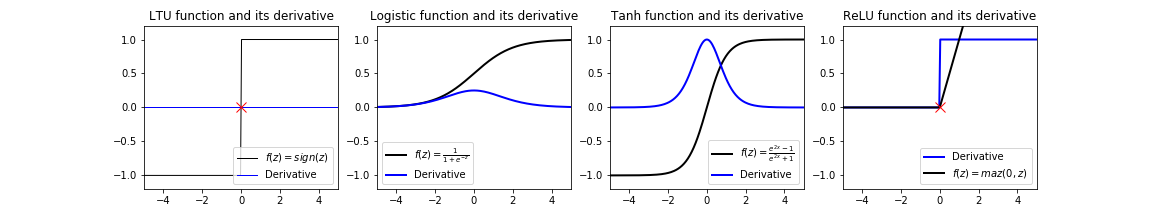
\includegraphics[width=1.0\textwidth]{activationFuncs.png}
\caption{Activation functions}
\label{fig:actFuncs}
\end{figure}
The reason that we need an activation function because each activation function is a nonlinear function and $\left(\sum_{i=0}^{n}x_i \times w_i\right)$ is a linear function. By chaining the $\left(\sum_{i=0}^{n}x_i \times w_i\right)$ to a nonlinear activation function $f$, the resulting function is a nonlinear function which can be used to fit any non-linear dataset.

To train a neuron is to obtain the set of weights $w_i$ such that the function $f(z)$ is best fit of the dataset. There are two common error functions that are used to measure the error of the expected output value $y_i$ of a sample $x_i$ and the estimated output value $\hat{y}$ returned from the model: the mean square error (MSE) function and the mean absolute error (MAE) function:
\begin{equation}
MSE = \frac{1}{m}\sum_{i=1}^{m}(\hat{y}^i - y^i)^2 
\end{equation}
\begin{equation}
MAE = \frac{1}{m}\sum_{i=1}^{m}|\hat{y}^i - y^i|
\end{equation}
where m is the number of instances in the dataset, $x^i$ is a vector of all the input features of the $i^{ih}$ instance, and $y^i$ is the expected output value. To obtain the set of weights $w_i$ that is best fit to the dataset is to find the optimal solution for either MSE or MAE functions. 

Gradient descent algorithm is a popular method to find the optimal solution any convex function like MSE or MAE error functions. The gradient descent algorithm starts with an random weight vector $\vec{\mathbf{w}}$ and measures the local gradient of the error function with respect to the parameter weight vector $\vec{\mathbf{w}}$. Then it goes in the direction of descending gradient until the error function reaches to the minimum. Specifically, for a dataset $\mathbf{X}^{m \times n}$, in each iteration, the weight vector is computed as:
\begin{equation} \label{fullbatchweightComp}
\mathbf{\vec{w}}^{t+1} = \mathbf{\vec{w}}^t - \eta\nabla_{\mathbf{\vec{w}}}MSE(\mathbf{\vec{w}}) 
\end{equation}
where $\eta$ is a learning rate hyperparameter and
\begin{equation} \label{fullbatchGrad}
\nabla_{\mathbf{\vec{w}}}MSE(\mathbf{\vec{w}})= \frac{2}{m}\mathbf{X^T}(\mathbf{X}\vec{\mathbf{w}} - \mathbf{y})
\end{equation}
The (\ref{fullbatchweightComp}) and (\ref{fullbatchGrad}) is called batch gradient descent algorithm which uses the entire training dataset to compute the gradient at every step and it is expensive. The least expensive gradient descent is used stochastic gradient descent (SGD) algorithm which randomly picks a sample in every step and computes the gradients only on that random instance. In between, there is a algorithm called mini-batch gradient descent algorithm which compute the gradients based on small random sets of instances call mini-batches. 

The above discussion is for training a neuron. A neural network is composed of an input layer, an output layer, and number of hidden layers in between the input and output layer. Each neuron in a hidden layer is fully connected to the neurons in the next layer. Backpropagation algorithm is used to train a neural network. The backprogation is a two-stage process: forward pass and backward pass as shown in Figure \ref{fig:NN}. Starting with random values of all the weight, below is the outline steps of the backpropagation algorithm:
\begin{enumerate}
\item The inputs are passed to the input layer which sends these inputs to the first hidden layer. The algorithm computes the outputs of all the neurons in this layer. Then the results are passed on to the next hidden layer and so on until the computed results reach to the output layer. This is a forward pass. All the intermediate results are recorded since these computed results are needed for the backward pass.
\item Using a loss function, the algorithm measures the network's output error. It then computes how much each output connection contributed to the error.
\item The algorithm then calculates error gradient for each neuron in the hidden layer below the output layer and propagating the error gradient backward to the hidden layers until the algorithm reaches to the input layer.
\item Using these gradient errors and gradient descent method, the algorithm to update all the connection weights in the network. 
\end{enumerate}
The algorithm iterates these steps until the error of the network converges to the acceptable minimum value.

\subsection{Convolutional neural network architecture} \label{CNN}
In this project, we use the convolutional neural network (CNN) to learn the Boltzmann equation's collision operator. As shown in Figure \ref{fig:CNN}, a CNN consists of input layers, convolutional layers, pooling layers, fully-connected layers, activation functions, and output layers. Comparing with the fully-connected neural network, a CNN architecture introduces two new building block: convolutional layers and pooling layers. Below, we briefly describes the structure of a convolutional layer and a pooling layer.

In a convolutional layer, neurons are only partially connected with the neurons in the previous layer: each neuron is only connected to the neurons located within a small rectangle in the previous layer. This small window is called the receptive field. This architecture allows the CNN to focus on small low-level features in the preceding hidden layer, then assemble them into larger higher-level features in the next hidden layer, and so on. This receptive field window is then moved across the layer horizontally and vertically with a step size called the stride length. All the receptive field share the same set of weights known as the kernel or filter. The outputs from this filter is known as a feature map. A convolutional layer may have multiple filters with each filter has different weights allowing a convolutional layer to detect multiple features of the inputs. 

After the convolutional layer is the pooling layer which is used to subsample the input image. Just like the convolutinal layer structure, each neuron in a pooling layer is connected to a number of neurons located in a small window receptive field in the previous layer. The difference between a convolutional layer and a pooling layer is that a pooling layer does not have the weights associated with a filter. The pooling layer uses an aggregate function such as max or mean to compute the maximum or the average among the neurons in a receptive field in a previous layer that are connected to a neuron in a pooling layer.

After the convolutional and pooling layers, the remaining part of a CNN is the fully-connected layers and an output layer. The fully-connected layer architecture was discussed in section \ref{FCNN}.

\begin{figure}
\centering
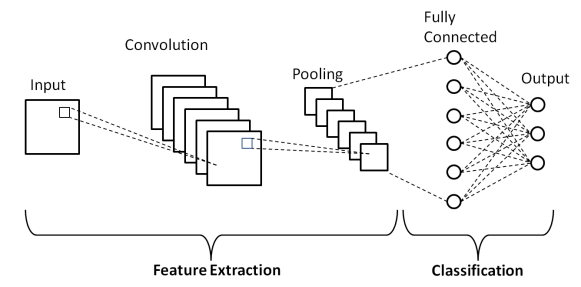
\includegraphics[width=1.0\textwidth]{CNN-architecture.png}
\caption{A basic convolutional neural network diagram}
\label{fig:CNN}
\end{figure}

\section{Using fully-connected autoencoder and convolutional neural network to learn the Boltzmann equation solutions and collision operator.}
In this section, we will describe the autoencoder and convolutional neural network architectures and how the these neural networks are trained and used to learn the Boltzmann equation data solution and the Boltzmann collision operator. We use Python numerical, Keras, and TensorFlow packages to develop and train autoencoders and CNN neural networks. One can refer to appendix A, B, and C for the detail of how we use the software tools, language, and training environment for this project. 

\subsection{The Boltzmann equation's solution dataset} \label{dataset}
In the following, we will discuss the method of generating the solution dataset of the Boltzmann equation using the numerical methods described in section \ref{BoltzSol}. This solution dataset will be used to train the autoencoders and CNN neural networks for learning the Boltzmann equation's solutions and collision operator. The solution data is obtained based on solving the spatially homogeneous equation (\ref{BoltzHomo}): $\frac{\partial}{\partial t}f(t,\vec{v}) = I[f](t, \vec{v})$. Below are the steps of generating the solution dataset:
\begin{itemize}
	\item Macroparameters of two homogeneous Gaussians are randomly generated and consecutively normalized so that the sum of Gaussians has unit density, zero bulk velocity, and pre-selected values of temperature of 0.5 and 0.2. The sum of two homogeneous Gaussians is used as the initial data for the solution.
	\item Equation \ref{BoltzHomo} is solved by \cite{Alekseenko4} for each set of randomly generated initial data. As the solutions are evolving in time, they are saved at even intervals of time. The computed solutions were saved in the files which will be used to construct the dataset for autoencoders and convolutional neural networks.
	\item The solutions were computed on $41^3$ discrete points. Due to the fact that solutions are very small near the boundary, a number of discrete points can be removed from the solution for analysis. The truncated solution has $31^3$ discrete points and the dataset has about 28,147  generated solutions.
	\item Loading all solution files into the memory for training the neural networks are time consuming. Instead, we have developed a software tool written in Python named \emph{ProcSolData.py} to put all the solution data into a compressed Pickle file for faster loading of the solution dataset into the computer memory.
	
\end{itemize}

\subsection{Learning solution data using autoencoders} \label{ae}
Figure \ref{fig:ae} shows a typical fully connected autoencoder architure. In an autoencoder, the number of neurons in an input layer is always equal to the number of neurons in the output layer. An autoencoder composes of two submodels: an encoder and a decoder.
\begin{figure}
\centering
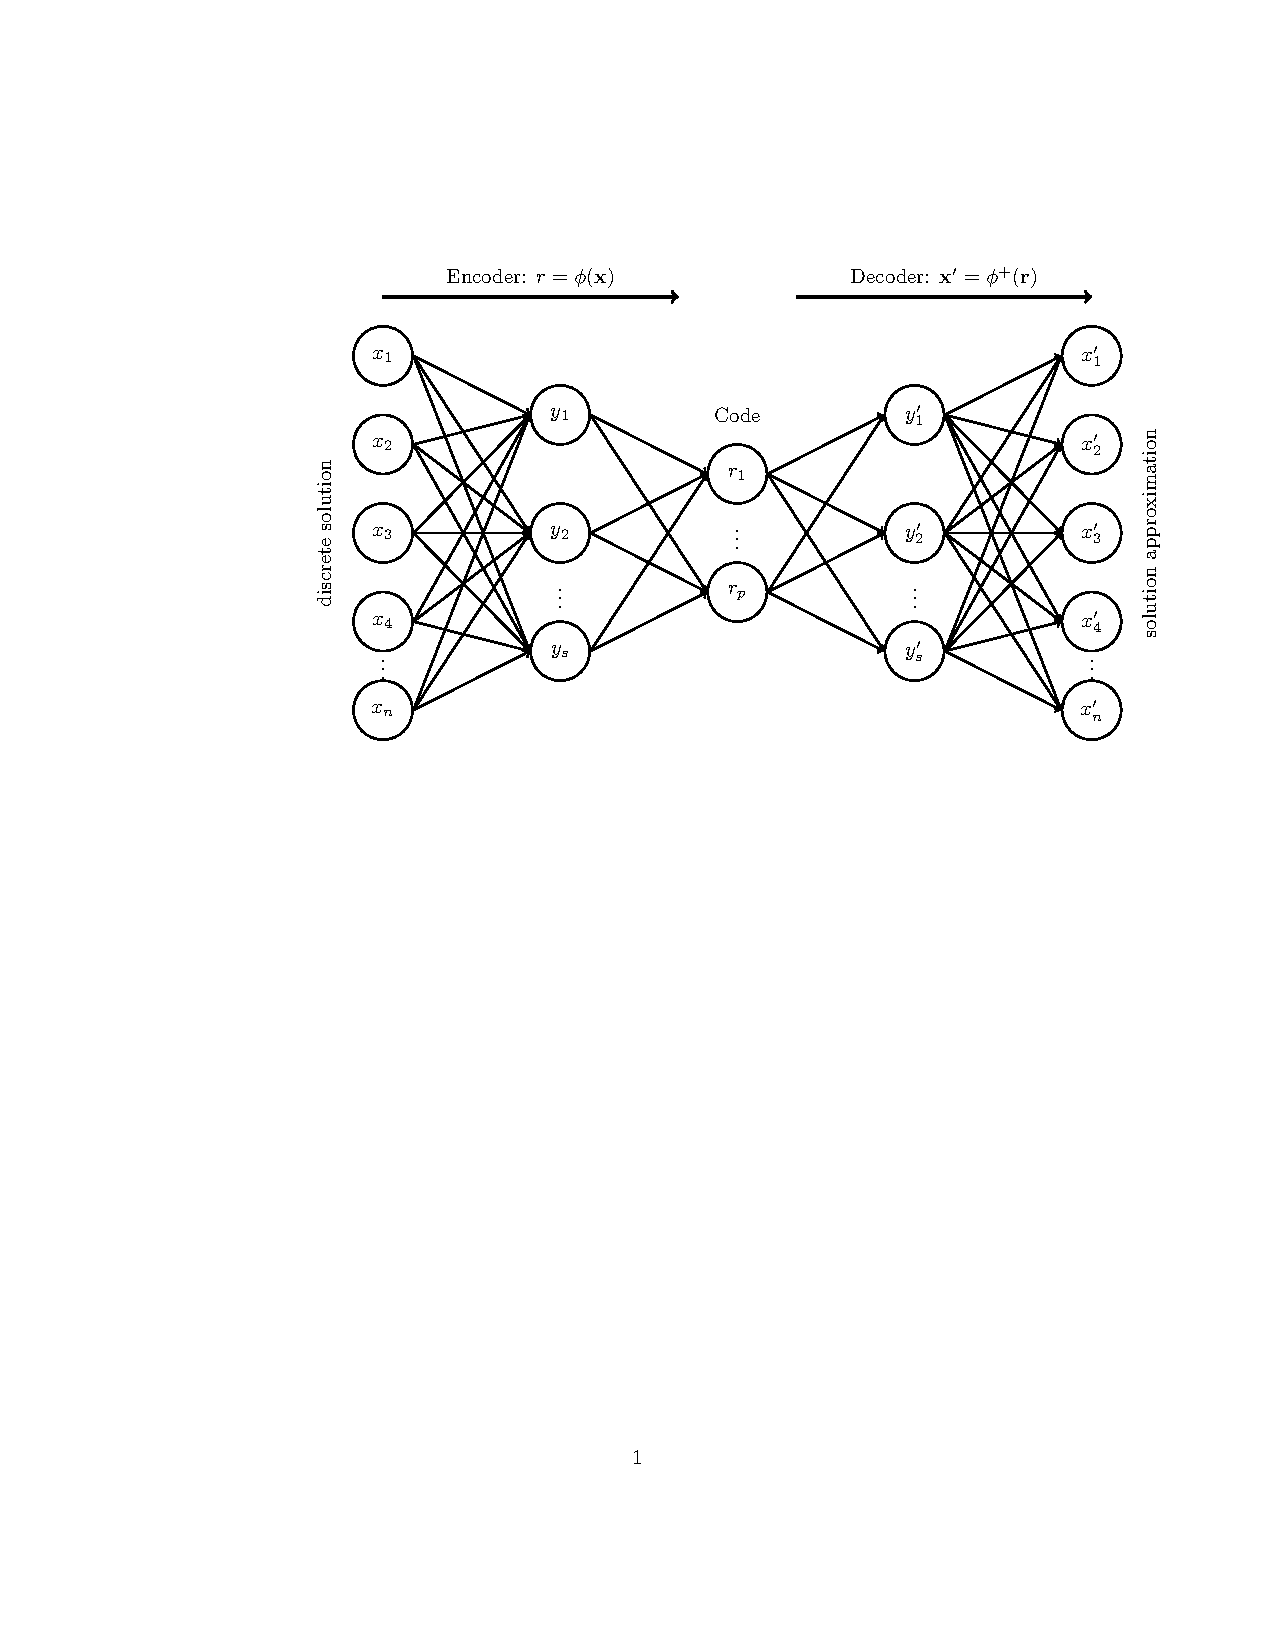
\includegraphics[width=1.0\textwidth]{Autoencoder.pdf}
\caption{A typical autoencoder architecture. An autoencoder composes of an encoder and a decoder. The encoder maps the input data to the code and the decoder reconstructs the inputs from the coding data}
\label{fig:ae}
\end{figure} 
The encoder model maps the inputs of higher dimension to a much lower dimensional data called the code. Then the coding data are fed into the decoder and the decoder reconstructs to output as the approximations of  inputs. The dimension of the code is much smaller than the dimension of the input. Autoencoder can be used to approximate the solutions of the Boltzmann equation as shown in the Figure \ref{fig:ae}. The encoder $r = \phi()\mathbf{x})$ maps discrete solutions to the code. The code is the input of the decoder $\mathbf{x'}=\phi^+(\mathbf{r})$ and the output of the decoder is the approximation of the solution data.


\subsubsection{Learing solution data using autoencoders and denoising encoders}
In this section, we will discuss the results of using autoencoders to learn the Boltzmann equation solutions. \emph{LearnSolData.py} code and \emph{settings.txt} setting file are used to construct different autoencoders. The dataset as described in section \ref{dataset} is used to train the autoencoders.  Following are the features of the autoencoders that we use to learn the Boltzmann equation solutions:
\begin{itemize}
	\item There are 28,147 solution data in the sample dataset. We used 90\% of samples for training and 10\% for validation.
	\item The input layer has 29,791 input neurons and the output layer also has the same number of neurons.
	\item For hidden layers, we used 1, 3, and 5 hidden layers.
	\item For code length, we used code length of 16, 32, and 64.
	\item For optimizer, we use Adam (\emph{adaptive moment estimation}) which is a faster optimizer than a regular gradient descent optimizer.
	\item For activation function, we used ReLU.
	\item For the loss function, MAE is used.
\end{itemize}
Table \ref{table:ae} below shows the accuracy of different autoencoders with various hidden layers and code lengths.

\begin{table} [h!]
\centering
\begin{tabular}{c|c|c|c|c|c|c|c|c|c}
	Hidden Layers & 1 & 1 & 1 & 3 & 3 & 3 & 5 & 5 & 5 \\
	\hline
	Code Length & 16 & 32 & 64 & 16 & 32 & 64 & 16 & 32 & 64 \\
	\hline
	Accuracy, MAE & 0.78 & 0.78 & 0.78 & 0.97 & 0.98 & 0.99 & 0.99 & 0.99 & 0.99
\end{tabular}
\caption{Accuracy of autoencoders with different number of hidden layers and code length.}
\label{table:ae}
\end{table}
We can add noise to the inputs and train the autoencoders to learn the features of the data and still able to recover the original inputs. These autoencoders are called denoising encoders. The denoising encoders have the same architectures as descirbed above for reqular encoders except we add 10\%, 15\%, 20\%, and 25\% noises to the inputs before training the encoders. The  Following is the results of training  denoising autoencoders with three hidden layers: 
\begin{table} [h!]
\centering
\begin{tabular}{c|c|c|c|c}
	Hidden Layers & 3 & 3 & 3 & 3 \\
	\hline 
	Code Length & 32 & 32 & 32 & 32 \\
	\hline
	Noise & 10\% & 15\% & 20\% & 25\% \\ 
	\hline
	Accuracy & 0.98 & 0.98 & 0.98 & 0.98
\end{tabular}
\caption{Accuracy of autoencoders with noises added to the inputs}
\label{table:ae_noise}
\end{table}

\noindent From table \ref{table:ae} and table \ref{table:ae_noise}, we have the following observations:
\begin{itemize}
	\item For autoencoders which have one hidden layer, the accuracy scores are low: 0.78. In this case, these autoencoders are underfitting.
	\item For autoencoders which have three hidden layers, the accuracy scores are very good. However, with code length of 64, the accuracy score is 0.98.
	\item For autoencoders which have five hidden layers, the accuracy scores improve slightly comparing with the autoencodes with three hidden layers.
	\item Adding noise to the inputs, the accuracy scores is still the same as if no noises are added to the inputs.  
\end{itemize}
Among these autoencoders, the autoencode with three hidden layers and code length 32 is probably is the best choice model. The second choice is the autoencoder with three hidden layers and code length 16 because the model is less complex, faster to train and compute, and the accuracy score is still about 0.98.

\subsubsection{Using trained autoencoder model to predict and visualize predicted solutions} \label{ae_visulize}
After training autoencoders, we can use these trained autoencoders to predict, visualize, and compare the computed solutions with the predicted solutions. \emph{predict\_viz\_gui.py} is the GUI (Graphical User Interface) program written in Python as shown in Figure \ref{fig:PredictVisualize1}. This GUI program allows an user to load different autoencoder and denoising autoencoder trained models and either randomly select number of solution data or specifically choose a solution data for predicting and visualizing the predicted solution. 
\begin{figure}[h!]
	\centering
	\includegraphics[width=1\textwidth]{PredictVisualize.png}
	\caption{GUI program for predicting and visualizing a Boltzmann solution}
	\label{fig:PredictVisualize1}
\end{figure}

Figure \ref{fig:Sol190} shows the graphs that a trained autoencoder predicts a seen solution and the error graph shows the error is about 5\%. Figure \ref{fig:Sol508} shows the graphs for the solution that the model has not seen it before and the error graph shows the error is about 1\%.

\begin{figure}[h]
	\centering
	\includegraphics[width=.99\textwidth]{Sol_predict_190.png}
	\caption{An autoencoder that is used to predict a solution that the model has seen the solution before.}
	\label{fig:Sol190}
\end{figure}

\begin{figure}[h]
	\centering
	\includegraphics[width=.99\textwidth]{Sol_predict_508.png}
	\caption{An autoencoder that is used to predict a solution that the model has not seen it before.}
	\label{fig:Sol508}
\end{figure}

\subsection{Learing collision operator using convolutional neural network (CNN)}
In this section, we will describe the CNN architecture that we used to learn the collision operator, to use the trained model to predict and visualize the solutions, and to use the Euler method to solve the differential equation based on the spatially homogeneous equation as described in section \ref{BoltzEq}
\begin{equation}
\frac{\partial}{\partial t}f(t,\vec{v}) = I[f](t, \vec{v})
\end{equation}

We can also use autoencoder to learn the Boltzmann collision operator: $Q:\mathbb{R}^N\rightarrow\mathbb{R}^N$ which provides the derivatives of the velocity distribution
As shown in Figure \ref{fig:ColOpAE}, the Boltzmann collision operator is approximated by an autoencoder.
\begin{figure}[h]
	\centering
	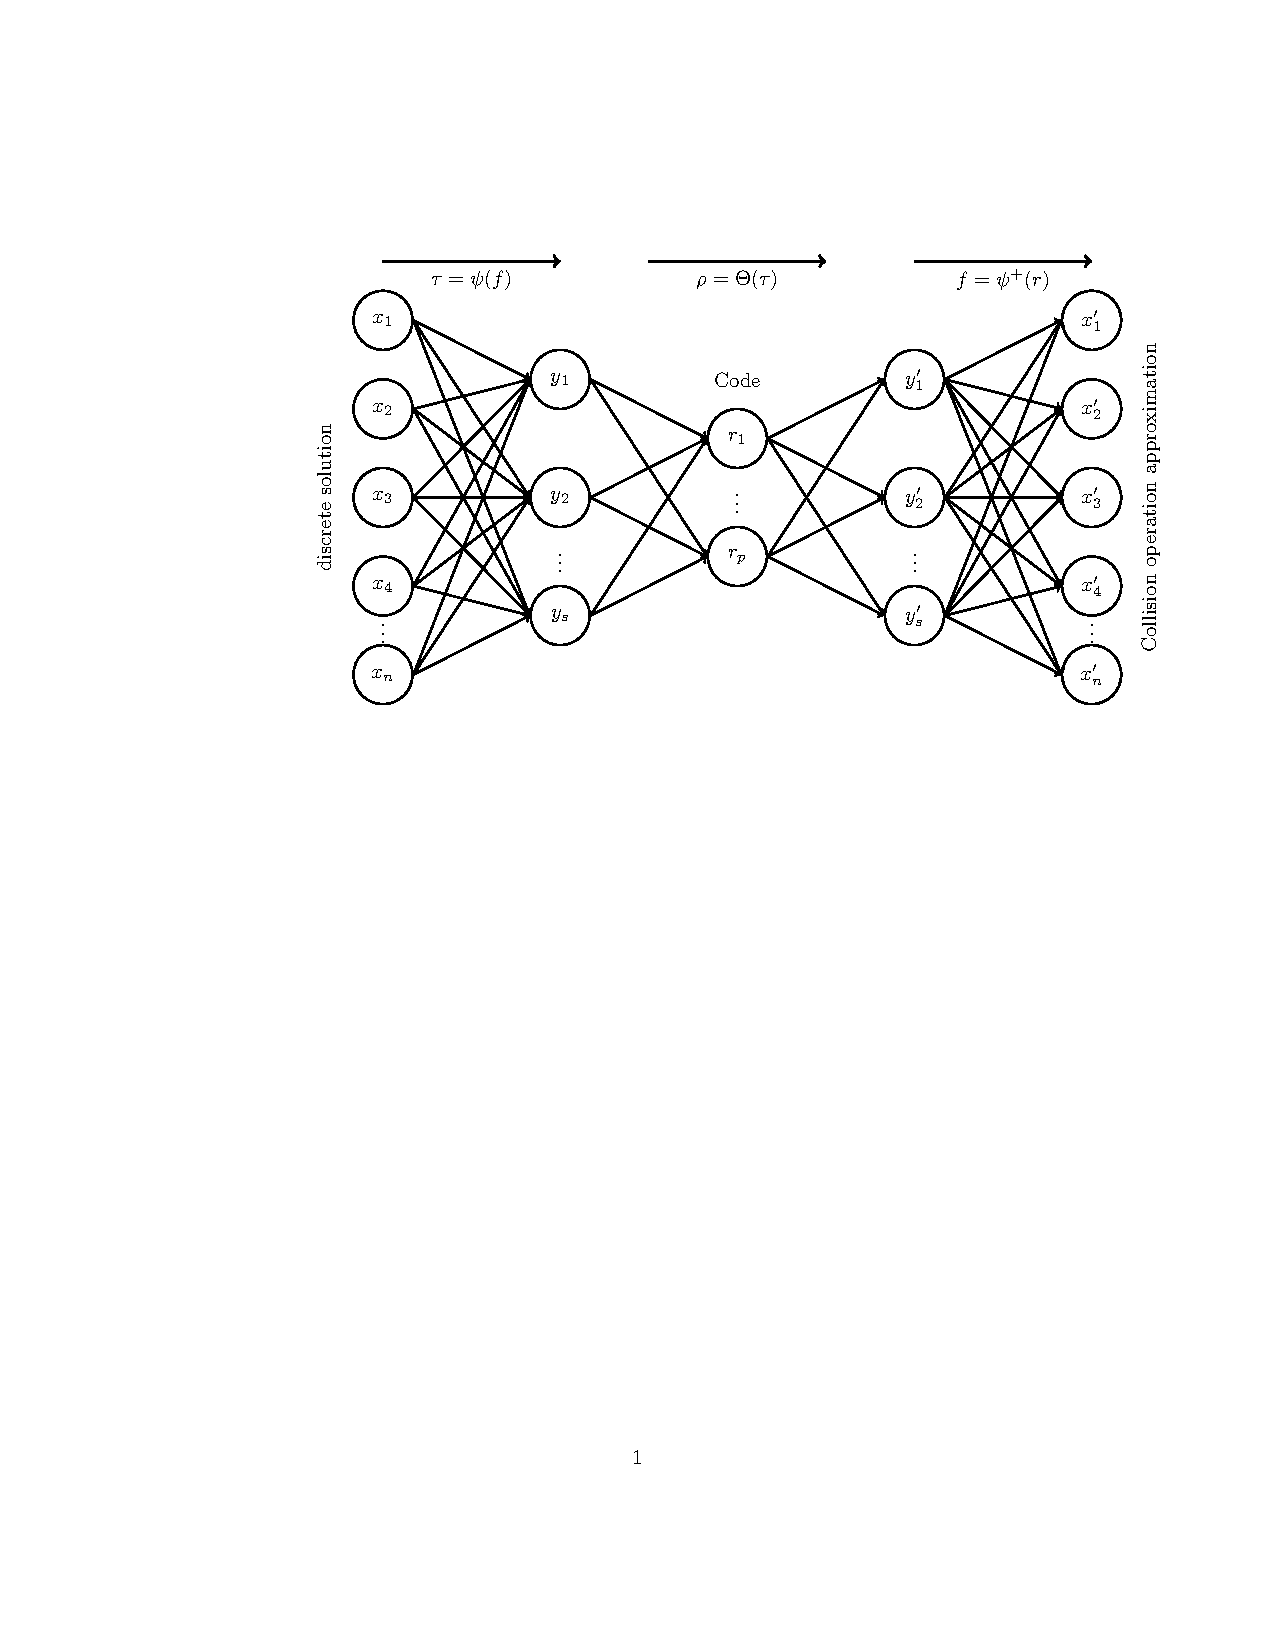
\includegraphics[width=.75\textwidth]{ColOpAE.pdf}
	\caption{An autoencoder that is used to approximate the Boltzmann collision operator}
	\label{fig:ColOpAE}
\end{figure}
\noindent To achieve fast evaluation, dimensions of the hidden layers should be significantly smaller than the size of input. Values predicted by the trained autoencoder can be used to approximate derivative of the solution and to do time integration. Formally, we can write
\begin{equation}
	\partial_t{\tau} = \partial_t(\psi(f)) = \frac{\partial\psi}{\partial f}:\frac{\partial f}{\partial t} = \frac{\partial\psi}{\partial f}:I(f) = \frac{\partial\psi}{\partial f}:I(\psi^+(\tau)) = \phi(\tau)
\end{equation}

\subsubsection{CNN architecture to learn collision operator} \label{learnCollOpCNN}
For learning collision operator, we found that the ReLU activation function did not perform well while traing the model to learn the collision operator because the ReLU has a zero slope in the negative region. To solve this problem, we use a variant of ReLU named as \emph{Leaky} ReLU which has a small positive slope in the negative region. Specifically, we use the \emph{parametric leaky} ReLU (PReLU) so that the slope of the ReLU in the negative region is adjusted accordingly during the training. Furthermore, the reason we chose the CNN because the CNN performs better than the fully-connected neural network. \emph{learn\_collision\_op\_cnn.py} is the source code written in Python to construct the CNN model and is trained with the dataset discussed in section \ref{dataset}. Below is the features of the CNN model that we use for training. One can refer to section \ref{CNN} for details of CNN architecture:

\begin{itemize}
	\item Rather than one dimension, the input data is three dimensions.
	\item The first hidden layer is a 3D convolutional layer with four filters with kernel size of (5,5,5).
	\item The second hidden layer is a 3D convolutional layer with eight filters with kernel size of (3,3,3).
	\item The third hidden layer is a 3D max pooling layer with kernel size of (2,2,2).
	\item The fourth hidden layer is a 3D convolutional layer with 16 filters with kernel size of (3,3,3).
	\item The fifth hidden layer id 3D max pooling layer with kernel size of (2,2,2).
	\item the sixth hidden layer is a 3D convolutional layer with 32 filters with kernel size of (3,3,3).
	\item The last hidden layer is a fully-connected layer with the one dimensional input.
	\item For activation function, we used the PReLU activation function as discussed above.
	\item For the loss function, we used the MAE loss function.
	\item For the optimizer, we used Adamax optimizer.
\end{itemize}
Unlike training an autoencoder which takes less than an hour on a fast computer, training a CNN model to learn collision operator can take multiple days and the accuracy is about 80\% to 90\%.

\subsubsection{Using trained CNN model to predict and visualize collision operator solutions}
After training a CNN model to learn collision operator, we can use the trained CNN model to predict a collision operator value given a Boltzmann equation solution. The same GUI program as discussed in section \ref{ae_visulize} is used to predict and visualize the predicted solutions. Figure \ref{fig:CollOp_167} and \ref{fig:CollOp_508} shows the CNN model can predict a seen solution and unseen solution with accuracy of 80\% and 90\% respectively.

\begin{figure}[h]
	\centering
	\includegraphics[width=.99\textwidth]{CollOp_167.png}
	\caption{A trained CNN model that is used to predict a seen solution.}
	\label{fig:CollOp_167}
\end{figure}

\begin{figure}[h]
	\centering
	\includegraphics[width=.99\textwidth]{CollOp_508.png}
	\caption{A trained CNN model that is used to predict an unseen solution.}
	\label{fig:CollOp_508}
\end{figure}

\subsubsection{Solving Boltzmann spatially homogeneous equation numerically}
With the homogeneous equation \ref{BoltzHomo} and a given initial value, we can use  the trained CNN model that learn the collision operator to predict the collision operator values and  numerically approximate the solution values for equation \ref{BoltzHomo} using Euler method:
\begin{equation} \label{Euler}
f_{k+1}= f_k + \Delta t \cdot I(t_k)
\end{equation}
After obtaining computed solution values numerically, we compute the moments of computed solution data as:
\begin{equation} \label{moments}
M_i = \int_{\mathbb{R}^3} (v_i - \tilde{v_i})^n f(v)dv
\end{equation}
where $n=2,3,4,5,6$ and $i=1,2,3$ for computing second moment, third moment, forth moment, fifth moment, and sixth moment. To numerically compute  equation \ref{Euler} and \ref{moments} and visualize the results, we developed two separate programs:  
\begin{itemize}
	\item \emph{NN\_Boltzmann\_solver.py} is a GUI program as shown in Figure \ref{fig:solver1}. Rhis GUI program lets user to choose a CNN model and an intial value. After that, the user can clicks on the \emph{Compute Solution} button to let the program solves the spatially homogeneous equation \ref{BoltzHomo} based the Euler equation \ref{Euler}, computes the moments based on equation \ref{moments}, and saves the moment results into a file.
	\item \emph{SpatHomRelaxROMM41Trim0\_VBA\_01.xlsm} is a EXEL-Visual Basic GUI program as shown in Figure \ref{fig:EXCEL1}. This program visualizes the moment results that are computed from the \emph{NN\_Boltzmann\_solver.py} program as described above.
\end{itemize}

\begin{figure}[h!]
	\centering
	\includegraphics[width=1\textwidth]{Solver.png}
	\caption{A GUI program uses a CNN model to predict solutions, solve the spatially homegeneous Boltzmann equation, and compute moments. }
	\label{fig:solver1}
\end{figure}

\begin{figure}[h!]
	\centering
	\includegraphics[width=1\textwidth]{EXCEL.png}
	\caption{An EXCEL Visual Basic program to plot computed moments and moments of solution data}
	\label{fig:EXCEL1}
\end{figure}

Figure \ref{fig:Moments_seen} and Figure \ref{fig:Moments_unseen} show the second, third, and forth moments of spatially homogeneous solutions both the seen and unseen solutions. From these figures, we can see that the solutions reach to the correct steady state except at the end there are some violations of the conservation of mass.

\begin{figure}[h]
	\includegraphics[width=.30\textwidth]{M2_seen}
	\hfill
	\includegraphics[width=.30\textwidth]{M3_seen}
	\hfill
	\includegraphics[width=.30\textwidth]{M4_seen}
	\caption{Relaxation of second, third, forth moments in seen solutions of spatially homogeneous problem}
	\label{fig:Moments_seen}	
\end{figure}

\begin{figure}[h]
	\includegraphics[width=.30\textwidth]{M2_unseen}
	\hfill
	\includegraphics[width=.30\textwidth]{M3_unseen}
	\hfill
	\includegraphics[width=.30\textwidth]{M4_unseen}
	\caption{Relaxation of second, third, forth moments in unseen solutions of spatially homogeneous problem}
	\label{fig:Moments_unseen}	
\end{figure}

\section{Computational efficiency and memory requirements of neural network methods for computing the solutions of Boltzmann equation } \label{efficiency}
\subsection{Time to predict solutions using autoencoder model and CNN models}
We used to autoencoders and CNN models to predict several solutions estimate the average time for predicting a solution. We use the GUI program as show in Figure \ref{fig:PredictVisualize1} and specifically select a solution data for an autoencoder or a CNN model to compute the time the trained model to predict a solution.  Following are the results:
\begin{table} [h!]
	\centering
	\begin{tabular}{c|c}
		Autoencoder & CNN model \\
		\hline
		0.0156288 & 0.171838 \\
		\hline
		0.0312495 & 0.140569 \\
		\hline 
		0.0312864 & 0.124941 \\
		\hline
		0.0312442 & 0.109284 \\
		\hline
		0.0278949 & 0.124950 \\
		\hline
		0.0312438 & 0.175418 \\
		\hline
		0.0352723 & 0.109351 \\
		\hline
		0.0311989 & 0.124971 \\
		\hline
		0.0312817 & 0.124930 \\
		\hline
		0.0261788 & 0.109310 \\
		\hline
		0.0312540 & 0.171805 \\
		\hline
		0.0312030 & 0.124971 \\
		\hline
		0.0312209 & 0.124970 \\
		\hline
		0.0156220 & 0.109307 \\ 
		\hline
		0.0312440 & 0.109319 \\
		\hline
		0.0312442 & 0.109392 \\
		\hline
		0.0312933 & 0.109391 \\
		\hline
		0.0311977 & 0.125331 \\
		\hline
		0.0312070 & 0.109349 \\
		\hline
		0.0312058 & 0.124971 \\
		\hline
		0.0312464 & 0.109327 \\
		\hline
	\end{tabular}
	\caption{Time predicting a solution for autoencoder and CNN models }
	\label{table:time}
\end{table}


\begin{itemize}
	\item For an autoencoder, the average time it takes to predict a solution is about 0.029458 second based on results from Table \ref{table:time}
	\item For a CNN model, the average time it takes to predict a solution is 0.121249 second based on results from Table \ref{table:time}. 	
\end{itemize}
The reason that it takes longer time for a CNN model to predict a solution comparing with an autoencoder is that a CNN model has a lot more weights than an encoder.

\subsection{Computer memory requirements for autoencoder and CNN models}
In this section, we will discuss the memory requirements for autoencoder and CNN models. As mentioned in \ref{dataset} section, the solution size of a solution is $31^3 = 29791$ which is the input for autoencoder and CNN models. We will discuss only for the memory required to load a trained model for testing or predicting and not for the memory required to train a model. Training a neural network model requires much more memory than loading a trained model for testing.

\subsubsection{Estimate memory requirements for an autoencoder model}
After loading a autoencoder, we can call the function \emph{summary()} method provided by Python to obtain number of layers, input shape, output shape, and number of parameters used in the model. Below is the summary information:
\verbatiminput{ae_model_summary.txt}

As discussed in section \ref{ae}, an autoencoder is composed of an encoder and a decoder. This summary is for an autoencoder with three hidden layers with code length of 32. As shown in the summary, there are $3,847,295$ trainable parameters needed for this autoencoder. One can refer any neural network book to understand how to compute number of parameters for a fully-connected neural network. For example, we can compute the parameters for an encoder as:
\[
(29791 \times 64) + 64 + (64 \times 32) + 32 = 1908768 \ parameters
\]
where the first hidden layer has 64 neurons and second hidden layer has 32 neurons.
Assume each parameters is represented by a floating number and 4 bytes are needed for a floating number, then we can estimate the  memory required for an autoencoder is:
\[ 3847295 \times 4 = 15,389,189 bytes = 14.675 \ MB \]
\subsubsection{Memory requirements for a CNN model}
Below is the summary information for a CNN model:
\verbatiminput{cnn_model_summary.txt}
One can refer to section \ref{learnCollOpCNN} for the details of the CNN architecture that is used to generate this summary.
As we can see from this summary information, there are much more parameters to be used with CNN model than the autoencoder model.
From the summary, the dense layer has the most parameters. We can compute the parameters as follow:
\begin{itemize}
	\item For convolutional layer, the formula for computing number of parameters is:
	\[ weights = filters \times (kernel_w \times kernel_h \times kernel_d) \times filters_{n-1} + biases \]
	For example, we can the weights of layer conv3d\_1 as:
	\[ 8 \times (3 \times 3 \times 3) \times 4 + 8 = 872 \]
	\item For p\_re\_lu\_1 (PReLU) layer, we can compute number of parameters as:
	\[ 31^3 \times 8 = 238,328 \] 
	\item Dense (fully connected) layer, we can compute number of parameters as:
	\[ 29791 \times 10976 + 29791 = 327,015,807 \]
	
\end{itemize}
Assumed that 4 bytes are needed for each parameter, the memory required for this CNN model can be computed as:
\[ 327,486,770 \times 4 \ bytes \approx 1.25 \  GB \]

\section{Conclusion} \label{Conclusion}
In this project, we take a new approach to develop the deep autoencoder and convolutional neural networks to learn the solution data and collision operator respectively. We then use the trained convolutional neural network to numerically solve the spatially homogeneous Boltzmann equation using Euler method and plotted the results to compare the neural network results with the solution data. The result performance are good except that the results violated conservation of mass and energy at the end. For the future development, we will continue to look into issues of conservation of mass and energy to further improve the autoencoder and convolutional neural networks.
 
\appendix
\appendixpage
\section{Software language and tools for developing neural networks of learning Boltzmann equation}
Below are the software tools and language that we used to develop the neural networks:
\begin{itemize}
	\item Computer language: Python 3.8.5.
	\item Neural networks development tools: Scikit-Learn, Keras, and Tensorflow.
	\item IDE development environment: VisualCode.
	\item Microsoft Excel and Visual Basic.
\end{itemize}
For development environment, we use laptop/PC to develop the code, test and train autoencoders and CNN models with solution data for only small number of iterations (or epoches) to ensure the code is working properly. Below are the source code files that have been developed for this project:
\begin{itemize}
	\item \emph{settings.txt}: this text file contains the setting parameters that are used by other Python source files.
	\item \emph{ProcSolData.py}: this Python source code is used to read the solution data files into arrays. At the end, the code save these arrays into a pickle file. This pickle file is used by other source code to load the solution data back into arrays that are used to train the autoencoder and CNN models.
	\item \emph{LearnSolData.py}: this source file is used to train the autoencoders.
	\item \emph{learn\_collision\_operator\_cnn.py}: this source file is used to train CNN.
	\item \emph{predict\_viz\_gui.py}: this source file is a GUI (Graphical User Interface) program for a user to load an autoencoder or a CNN model to predict a solution.
	\item \emph{NN\_Boltzmann\_solver.py}: this source file is a GUI program for a user to load a CNN model to predict a initial value for the spatially homogeneous Boltzmann equation and apply Euler method to numerically to solve the spatially homogeneous Boltzmann equation given a predicted initial value.
	\item \emph{Utilities.py}: this file provides the utility functions that are used by other source code files.
	\item \emph{my\_readwrite.py}: this file is a library to provide functions to process solution data.
	\item \emph{my\_viz\_routines.py}: this file is to provide functions to help visualize the predicted solutions.	
	\item \emph{SpatHomRelaxROMM41Trim0\_VBA\_01.xlsm}: this is a EXCEL file with Visual Basic code to make the plots from the moment files that are created by the \emph{NN\_Boltzmann\_solver.py} program.
\end{itemize}

We can train autoencoders on the local PC because the training time won't take long. However, training CNN neural networks can take several hours or days to run and comsume a lot of computer resources, after testing the code working properly, we transfer python code and dataset to the XSEDE supercomputer to fully train autoencoders and CNN models as we describe in the next section.

\section{Training autoencoder and CNN model environments} 
After developed, tested, and trained the autoencoders and CNN models on local computer, for fully training autoencoders and CNN models with the solution data, we need to connect to the XSEDE supercomputer system to train the autoencoders and CNN models. Below are the programs that we used to transfer the code and solution dataset to the XSEDE system to train the autoencoders and CNN models. One can refer to document "StepsAccessToHPC.docx" written by professor Alekseenko for the detail of how to setup an XSEDE account, install PuTTY, FileZilla, etc. to connect to the XSEDE systems:
\begin{itemize}
	\item PuTTY tool to establish remote connection to the XSEDE system.
	\item Using FileZilla tool to connect to the XSEDE system and upload and download the files between the local PC and XSEDE directories.
	\item After the training completed on the XSEDE, we can download the trained neural network files to the local computer via FileZilla tool.
\end{itemize}

\section{GUI programs for predicting, visualizing, and solving the spatially homogeneous Boltzmann equation with the trained neural networks.}
\subsection{Predicting and visualizing the Boltzmann solution using trained autoencoders and CNN models.}
The \emph{predict\_viz\_gui.py} is a GUI program that is used to load either a trained autoencoder or a trained CNN model and predict a solution as shown in figure \ref{fig:PredictVisualize}
\begin{figure}[h!]
	\centering
	\includegraphics[width=1\textwidth]{PredictVisualize.png}
	\caption{GUI program for predicting and visualizing a Boltzmann solution}
	\label{fig:PredictVisualize}
\end{figure}

Below are the steps to generate the figure \ref{fig:PredictVisualize}
\begin{enumerate}
	\item Choose a \emph{Learn Solutions} or \emph{Learn Collision Operator CNN} radio button.
	\item Click on \emph{Select a model} button to select either an autoencoder or a CNN model to test.
	\item Click on \emph{Select data folder} button to choose a solution data folder to test.
	\item Click on \emph{Random Predicts} button to let the program to randomly select 20 solution data to predict. The program will fill the predicted solutions into the \emph{predicted solutions: click an item to visualize} list.
	\item User can click any predicted solution in the list to visualize the predicted solution as shown in figure \ref{fig:PredictVisualize}.	
\end{enumerate}
User can click on \emph{Predict one solution} button to specifically select a solution rather let the program randomly select solutions. After specifically select a solution, the program will predict and visualize the data.

\begin{figure}[h!]
	\centering
	\includegraphics[width=1\textwidth]{SolPredict.png}
	\caption{Graphically comparing a solution with a predicted solution}
	\label{fig:SolPredict}
\end{figure} 
\subsection{GUI programs to solve and visualize the spatially homogeneous Boltzmann equation}

There are two GUI programs \emph{NN\_Boltzmann\_solver.py program} and \emph{SpatHomRelaxROMM41Trim0\_VBA\_01.xlsm} that works together to numerially solve the spatially homogeneous Boltzmann equation based on Euler method.
\begin{figure}[h!]
	\centering
	\includegraphics[width=1\textwidth]{Solver.png}
	\caption{A GUI program uses a CNN model to predict solutions, solve the spatially homegeneous Boltzmann equation, and compute moments. }
	\label{fig:solver}
\end{figure}
Below are the steps of how to use the \emph{NN\_Boltzmann\_solver.py program} as shown in figure \ref{fig:solver}:
\begin{enumerate}
	\item Click on \emph{Select a CNN model} button to select a trained CNN model.
	\item Click on \emph{Select an initial value file} button to select an initial value value file from a solution folder.
	\item Click on \emph{Compute solution} to let the program to use the CNN model and the initial value file to predict a solution, apply the Euler method to iteratively solve the next value, compute the moments, and save the computed moments into a file.
\end{enumerate}

After the \emph{NN\_Boltzmann\_solver.py program} finished, the user will run the \emph{SpatHomRelaxROMM41Trim0\_VBA\_01.xlsm} to load the moment and solution files into the spreadsheet and use the Visual Basic programs to generate the plots to visually compare the computed moments and moments of solution data as shown in figure \ref{fig:EXCEL}. The \emph{NN\_Boltzmann\_solver.py program} is an EXCEL spreadsheet  with Visual Basic progams.

\begin{figure}[h!]
	\centering
	\includegraphics[width=1\textwidth]{EXCEL.png}
	\caption{An EXCEL Visual Basic program to plot computed moments and moments of solution data}
	\label{fig:EXCEL}
\end{figure}
 
\section{Documents and source code revision control}
We maintain source files, documents, and revisions in GitHub under \\ \href{https://github.com/tlatttt/Math698A-Thesis}{https://github.com/tlatttt/Math698A-Thesis}. Figure \ref{fig:GitHub} shows the source files and directories of this project on the GibHub. 
\begin{figure}[h!]
	\centering
	\includegraphics[width=1\textwidth]{GitHub.png}
	\caption{A screen shot of the source files, documents that are maintained on GitHub}
	\label{fig:GitHub}
\end{figure}

\pagebreak
\begin{thebibliography}{99}
	\bibitem{RarefiedGasD}M. Kogan, Rarefied gas dynamics, Plenum Press, 1969.
	\bibitem{IntroBoltz}Stewart Harris, An Introduction to the Theory of the Boltzmann Equation, 1971, 2004.
	\bibitem{Alekseenko1}A. Alekseenko and E. Josyula.  Deterministic Solution of the Boltzmann Equation Using a Discontinuous Galerkin Velocity Discretization. In 28th, International Symposium on Rarefied Gas Dynamics, 9-13 July 2012, Zaragoza, Spain, AIP Conferences Proceedings, page 8. American Institute of Physics, 2012.
	\bibitem{Alekseenko2}A. Alekseenko and E. Josyula.  Deterministic Solution Of The Spatially Homogeneous Boltzmann Equation Using Discontinuous Galerkin Discretizations In The Velocity Space. Journal of Computational Physics, 272(0): 170 – 188, 2014.
	\bibitem{Alekseenko3}A. Alekseenko, T. Nguyen, and A. Wood. A Deterministic-Stochastic Method For Computing The Boltzmann Collision Integral In O(Mn) Operations. Kinetic \& Related Models,11(1937-5093.2018.5.1211):1211, 2018.
	\bibitem{Alekseenko4}Alexander Alekseenko and Jeffrey Jimbacher. Evaluating High Order Discontinuous Galerkin Discretization of The Boltzmann Collision Integral In O(N2) Operations Using The Discrete Fourier Transform, 2019.
	\bibitem{LBM1} Peter Mora, Gabriele Morra and David A. Yuen. A concise python implementation of the lattic Boltzmann method on HPC for geo-fluid flow, Geophysical Journal International 2019.
	\bibitem{LBM2} Timm K\"{u}ger, Halim Kusumaatmaja, Alexandr Kuzmin, Orest Shardt, Goncalo Silva, and Erlend Magnus Viggen. The Lattic Boltzmann Method, Principles and Practice. Springer 2017
	\bibitem{WikiTheoryOfGas}Wikipedia, Kinetic theory of gases,https://en.wikipedia.org/wiki/Kinetic\_theory\_of\_gases.
	\bibitem{DSMC1}Fransis J. Alexender, Alejandro L. Garcia, The Direct Simulation Monte Carlo Method, Computer In Physics, Vol 11, Nov 1997.
	\bibitem{DSMC2}Lorenzo Pareschi, Giovanni Russo, An Introduction to Monte Carlo Methods for Boltzmann Equation, ESAIM Proceedings, 1999.
	\bibitem{DSMC3}A. A. Ganjaei and S. S. Nourazar, A new algorithm for the simulation of the boltzmann equation using the direct simulation monte-carlo method, Journal of Mechanical Science and Technology 23 (2009) 2861~2870.
	\bibitem{BirdGA1}Bird, G. A., “Approach to Translational Equilibrium in a Rigid Sphere Gas.” Physics of Fluids, Vol. 6, 1963, pp. 1518-1519.
	\bibitem{BirdGA2}Bird, G. A., Molecular Gas Dynamics and the Direct Simulation of Gas Flows, Charendon Press, Oxford, 1994.
	\bibitem{VVAristo} V. V. Aristo. Direct Methods for Solving the Boltzmann Equation and Study of Nonequilibrium flows, 2001.
	\bibitem{HandOnML}Anr\'{e}lien G\'{e}ron, Hands-on Machine Learning with Scikit-Learn, Keras \& TensorFlow, O'Reilley, 2019
	\bibitem{IntroML}Andreas C. Müller, Guido, Sarah. Introduction to Machine Learning with Python, 2017.
	\bibitem{DeepLearning}John D. Kelleher, Deep Learning, The MIT Press, 2019.
	\bibitem{Autoencoder1}Francois Chollet et al. Keras. https://github.com/fchollet/keras, 2015.
	\bibitem{NNmemory}Deep Learning For Computer Vision. Memory usage and computational considerations: http://imatge-upc.github.io/telecombcn-2016-dlcv/slides/D2L1-memory.pdf, 8 July 2016  
\end{thebibliography}
\end{document}